\chapter{Convex Sets, Functions and Cones and Polyhedral Theory}
In this chapter, we will cover all of the geometric prerequisites for understanding the theory of linear programming. We will use the results in this section to prove theorems about the Simplex Method in other sections.

\section{Convex Sets}
\begin{definition}[Convex Set] Let $X \subseteq \mathbb{R}^n$. Then the set $X$ is convex if and only if for all pairs $\mathbf{x}_1,\mathbf{x}_2 \in X$ we have $\lambda\mathbf{x}_1 + (1-\lambda)\mathbf{x}_2 \in X$ for all $\lambda \in [0,1]$.
\end{definition}

The definition of convexity seems complex, but it is easy to understand. First recall that if $\lambda \in [0,1]$, then the point $\lambda\mathbf{x}_1 + (1-\lambda)\mathbf{x}_2$ is on the line segment connecting $\mathbf{x}_1$ and $\mathbf{x}_2$ in $\mathbb{R}^n$. For example, when $\lambda = 1/2$, then the point $\lambda\mathbf{x}_1 + (1-\lambda)\mathbf{x}_2$ is the midpoint between $\mathbf{x}_1$ and $\mathbf{x}_2$. In fact, for every point $\mathbf{x}$ on the line connecting $\mathbf{x}_1$ and $\mathbf{x}_2$ we can find a value $\lambda \in [0,1]$ so that $\mathbf{x} = \lambda\mathbf{x}_1 + (1-\lambda)\mathbf{x}_2$. Then we can see that, convexity asserts that if $\mathbf{x}_1,\mathbf{x}_2 \in X$, then every point on the line connecting $\mathbf{x}_1$ and $\mathbf{x}_2$ is also in the set $X$. 

\begin{definition}[Positive Combination] Let $\mathbf{x}_1,\dots,\mathbf{x}_m \in \mathbb{R}^n$. If $\lambda_1,\dots,\lambda_m > 0$ and 
then 
\begin{equation}
\mathbf{x} = \sum_{i=1}^m\lambda_i\mathbf{x}_i
\end{equation}
is called a \textit{positive combination} of $\mathbf{x}_1,\dots,\mathbf{x}_m$.
\end{definition}

\begin{definition}[Convex Combination] Let $\mathbf{x}_1,\dots,\mathbf{x}_m \in \mathbb{R}^n$. If $\lambda_1,\dots,\lambda_m \in [0,1]$ and 
\begin{displaymath}
\sum_{i=1}^m\lambda_i = 1
\end{displaymath} 
then 
\begin{equation}
\mathbf{x} = \sum_{i=1}^m\lambda_i\mathbf{x}_i
\label{eqn:ConvexCombination}
\end{equation}
is called a \textit{convex combination} of $\mathbf{x}_1,\dots,\mathbf{x}_m$. If $\lambda_i < 1$ for all $i=1,\dots,m$, then Equation \ref{eqn:ConvexCombination} is called a \textit{strict convex combination}.
\end{definition}

\begin{remark} If you recall the definition of linear combination, we can see that we move from the very general to the very specific as we go from linear combinations to positive combinations to convex combinations. A linear combination of points or vectors allowed us to choose any real values for the coefficients. A positive combination restricts us to positive values, while a convex combination asserts that those values must be non-negative and sum to 1.
\end{remark}

\begin{example}
Figure \ref{fig:ConvexSets} illustrates a convex and non-convex set.
\begin{figure}[htbp]
\centering
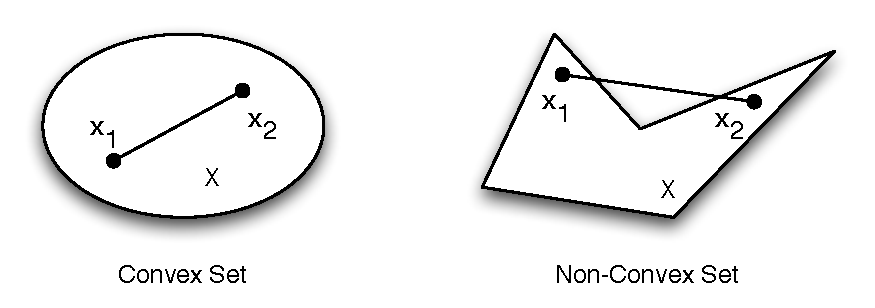
\includegraphics[scale=0.5]{ConvexSets.pdf}
\caption{Examples of Convex Sets: The set on the left (an ellipse and its interior) is a convex set; every pair of points inside the ellipse can be connected by a line contained entirely in the ellipse. The set on the right is clearly not convex as we've illustrated two points whose connecting line is not contained inside the set.}
\label{fig:ConvexSets}
\end{figure}
Non-convex sets have some resemblance to crescent shapes or have components that look like crescents.
\end{example}

\begin{theorem} The intersection of a finite number of convex sets in $\mathbb{R}^n$ is convex.
\end{theorem}
\begin{proof} Let $C_1,\dots,C_n \subseteq \mathbb{R}^n$  be a finite collection of convex sets. Let 
\begin{equation}
C = \bigcap_{i=1}^{n} C_i
\end{equation}
be the set formed from the intersection of these sets. Choose $\mathbf{x}_1,\mathbf{x}_2 \in C$ and $\lambda \in [0,1]$. Consider $\mathbf{x} = \lambda\mathbf{x}_1 + (1-\lambda)\mathbf{x}_2$. We know that $\mathbf{x}_1,\mathbf{x}_2 \in C_1,\dots,C_n$ by definition of $C$. By convexity, we know that $\mathbf{x} \in C_1,\dots,C_n$ by convexity of each set. Therefore, $\mathbf{x} \in C$. Thus $C$ is a convex set.
\end{proof}

\section{Convex and Concave Functions}
\begin{definition}[Convex Function] A function $f:\mathbb{R}^n \rightarrow \mathbb{R}$ is a convex function if it satisfies:
\begin{equation}
f(\lambda\mathbf{x}_1 + (1-\lambda)\mathbf{x}_2) \leq \lambda f(\mathbf{x}_1) + (1-\lambda)f(\mathbf{x}_2)
\end{equation}
for all $\mathbf{x}_1,\mathbf{x}_2 \in \mathbb{R}^n$ and for all $\lambda \in [0,1]$. 
\end{definition}
This definition is illustrated in Figure \ref{fig:QuadraticConvex}.
\begin{figure}[htbp]
\centering
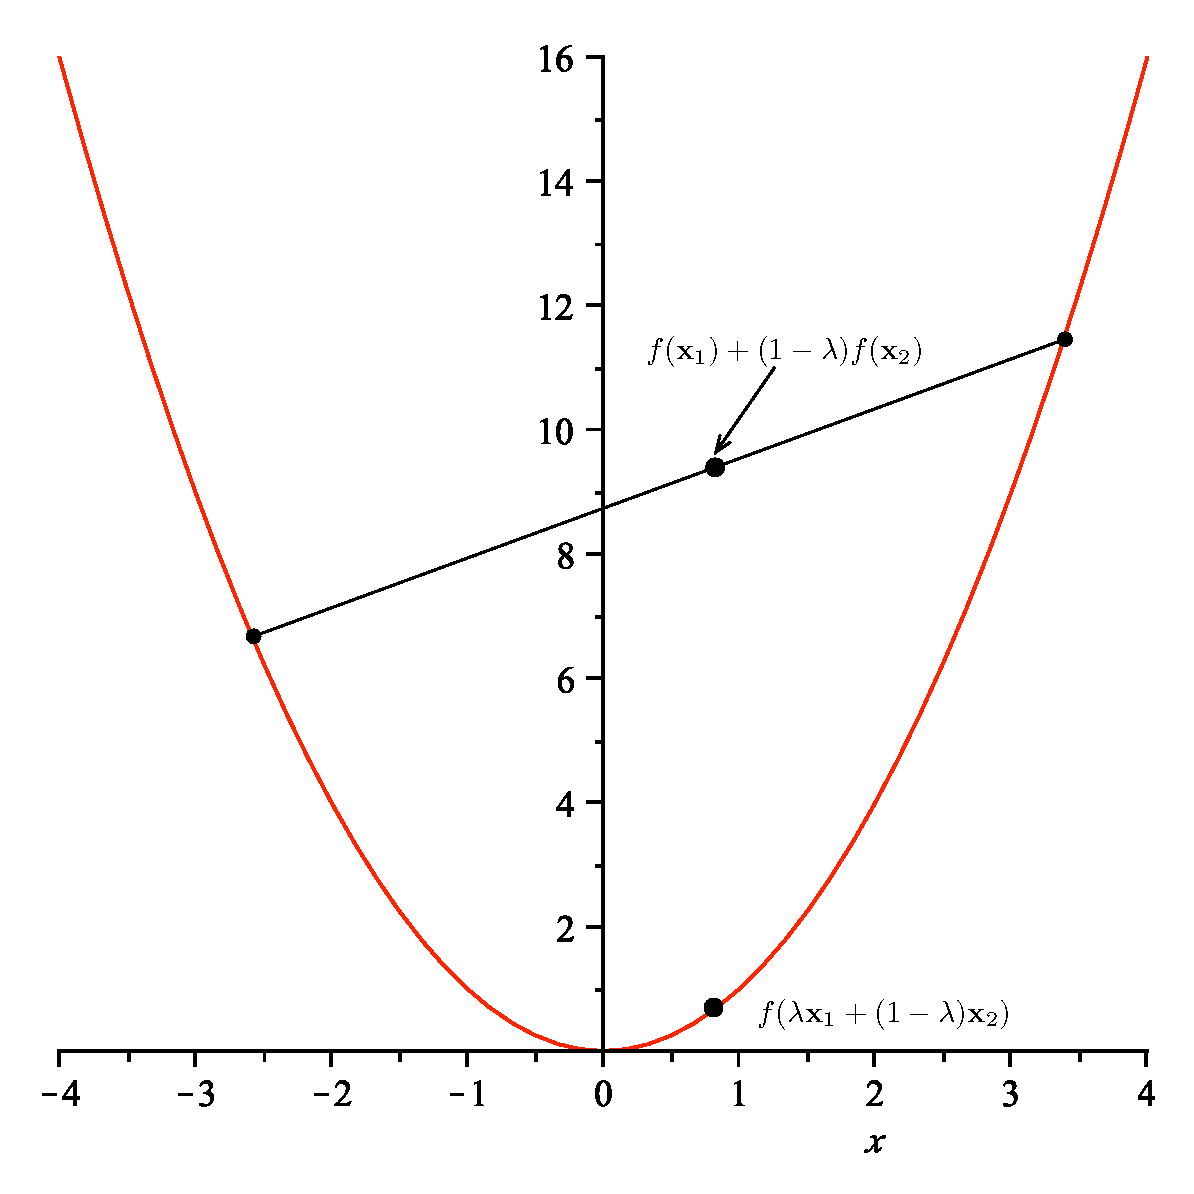
\includegraphics[scale=0.25]{QuadraticConvex.pdf}
\caption{A convex function: A convex function satisfies the expression $f(\lambda\mathbf{x}_1 + (1-\lambda)\mathbf{x}_2) \leq \lambda f(\mathbf{x}_1) + (1-\lambda)f(\mathbf{x}_2)$ for all $\mathbf{x}_1$ and $\mathbf{x}_2$ and $\lambda \in [0,1]$.}
\label{fig:QuadraticConvex}
\end{figure}
When $f$ is a univariate function, this definition can be shown to be equivalent to the definition you learned in Calculus I (Math 140) using first and second derivatives.
\begin{definition}[Concave Function] A function $f:\mathbb{R}^n \rightarrow \mathbb{R}$ is a concave function if it satisfies:
\begin{equation}
f(\lambda\mathbf{x}_1 + (1-\lambda)\mathbf{x}_2) \geq \lambda f(\mathbf{x}_1) + (1-\lambda)f(\mathbf{x}_2)
\end{equation}
for all $\mathbf{x}_1,\mathbf{x}_2 \in \mathbb{R}^n$ and for all $\lambda \in [0,1]$ \footnote{Thanks to Greg Ference and Veselka Kafedzhieva for catching a typo in this definition.}. 
\end{definition}
To visualize this definition, simply flip Figure \ref{fig:QuadraticConvex} upside down. The following theorem is a powerful tool that can be used to show sets are convex. It's proof is outside the scope of the class, but relatively easy. 
\begin{theorem} Let $f:\mathbb{R}^n \rightarrow \mathbb{R}$ be a convex function. Then the set $C = \{\mathbf{x} \in \mathbb{R}^n : f(x) \leq c\}$, where $c \in \mathbb{R}$, is a convex set. 
\label{thm:ConvexFunctionSet}
\end{theorem}

\begin{exercise} Prove the Theorem \ref{thm:ConvexFunctionSet}. [Hint: Skip ahead and read the proof of Lemma \ref{lem:HalfSpaceConvex}. Follow the steps in that proof, but apply them to $f$.]
\end{exercise}

\section{Polyhedral Sets}
Important examples of convex sets are polyhedral sets, the multi-dimensional analogs of polygons in the plane. In order to understand these structures, we must first understand hyperplanes and half-spaces. 

\begin{definition}[Hyperplane] Let $\mathbf{a} \in \mathbb{R}^n$ be a constant vector in $n$-dimensional space and let $b \in \mathbb{R}$ be a constant scalar. The set of points 
\begin{equation}
H = \left\{\mathbf{x} \in \mathbb{R}^n | 
\mathbf{a}^T\mathbf{x} = b\right\}
\end{equation}
is a \textit{hyperplane} in $n$-dimensional space. \textit{Note the use of column vectors for $\mathbf{a}$ and $\mathbf{x}$ in this definition.}
\end{definition}

\begin{example} Consider the hyper-plane $2x_1 + 3x_2 + x_3 = 5$. This is shown in Figure \ref{fig:HyperPlane}.
\begin{figure}[htbp]
\centering
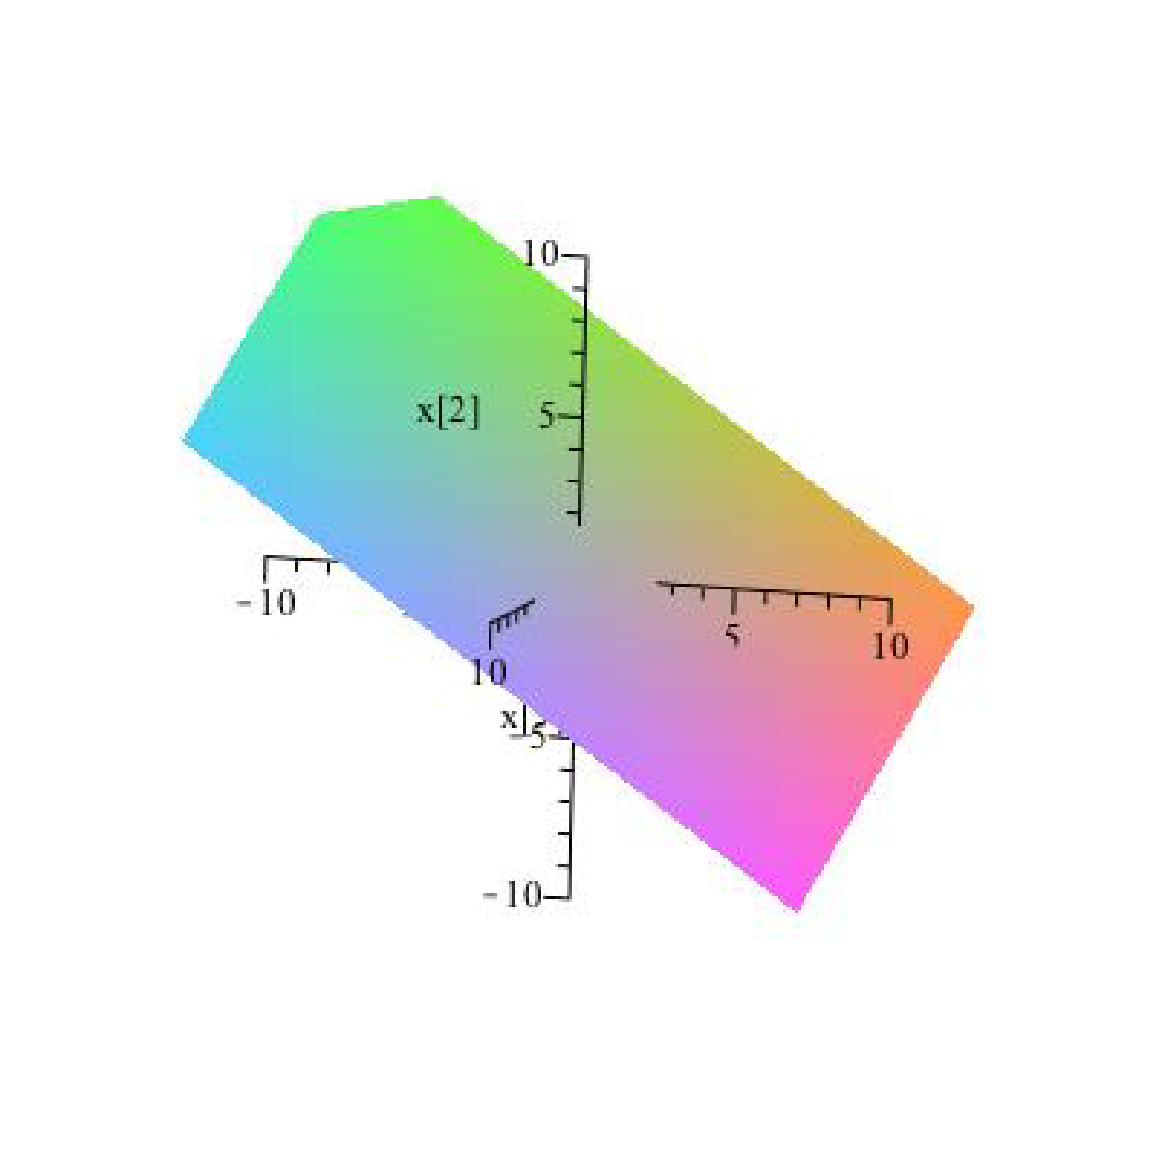
\includegraphics[scale=0.5]{HyperPlane.pdf}
\caption{A hyperplane in 3 dimensional space: A hyperplane is the set of points satisfying an equation $\mathbf{a}^T\mathbf{x} = b$, where $k$ is a constant in $\mathbb{R}$ and $\mathbf{a}$ is a constant vector in $\mathbb{R}^n$ and $\mathbf{x}$ is a variable vector in $\mathbb{R}^n$. The equation is written as a matrix multiplication using our assumption that all vectors are column vectors.}
\label{fig:HyperPlane}
\end{figure}
This hyperplane is composed of the set of points $(x_1,x_2,x_3) \in \mathbb{R}^3$ satisfying $2x_1 + 3x_2 + x_3 = 5$. This can be plotted implicitly or explicitly by solving for one of the variables, say $x_3$. We can write $x_3$ as a function of the other two variables as: 
\begin{equation}
x_3 = 5 - 2x_1 - 3x_2
\end{equation}
\end{example}

\begin{definition}[Half-Space] Let $\mathbf{a} \in \mathbb{R}^n$ be a constant vector in $n$-dimensional space and let $b \in \mathbb{R}$ be a constant scalar. The sets of points 
\begin{gather}
H_l = \left\{\mathbf{x} \in \mathbb{R}^n | \mathbf{a}^T\mathbf{x} \leq b\right\}\\
H_u = \left\{\mathbf{x} \in \mathbb{R}^n | \mathbf{a}^T\mathbf{x} \geq b\right\}
\end{gather} 
are the half-spaces defined by the hyperplane $\mathbf{a}^T\mathbf{x} = b$. 
\end{definition}
\begin{example} Consider the two dimensional hyperplane (line) $x_1 + x_2 = 1$. Then the two half-spaces associated with this hyper-plane are shown in Figure \ref{fig:HalfSpace}.
\begin{figure}[htbp]
\subfigure[$H_l$]{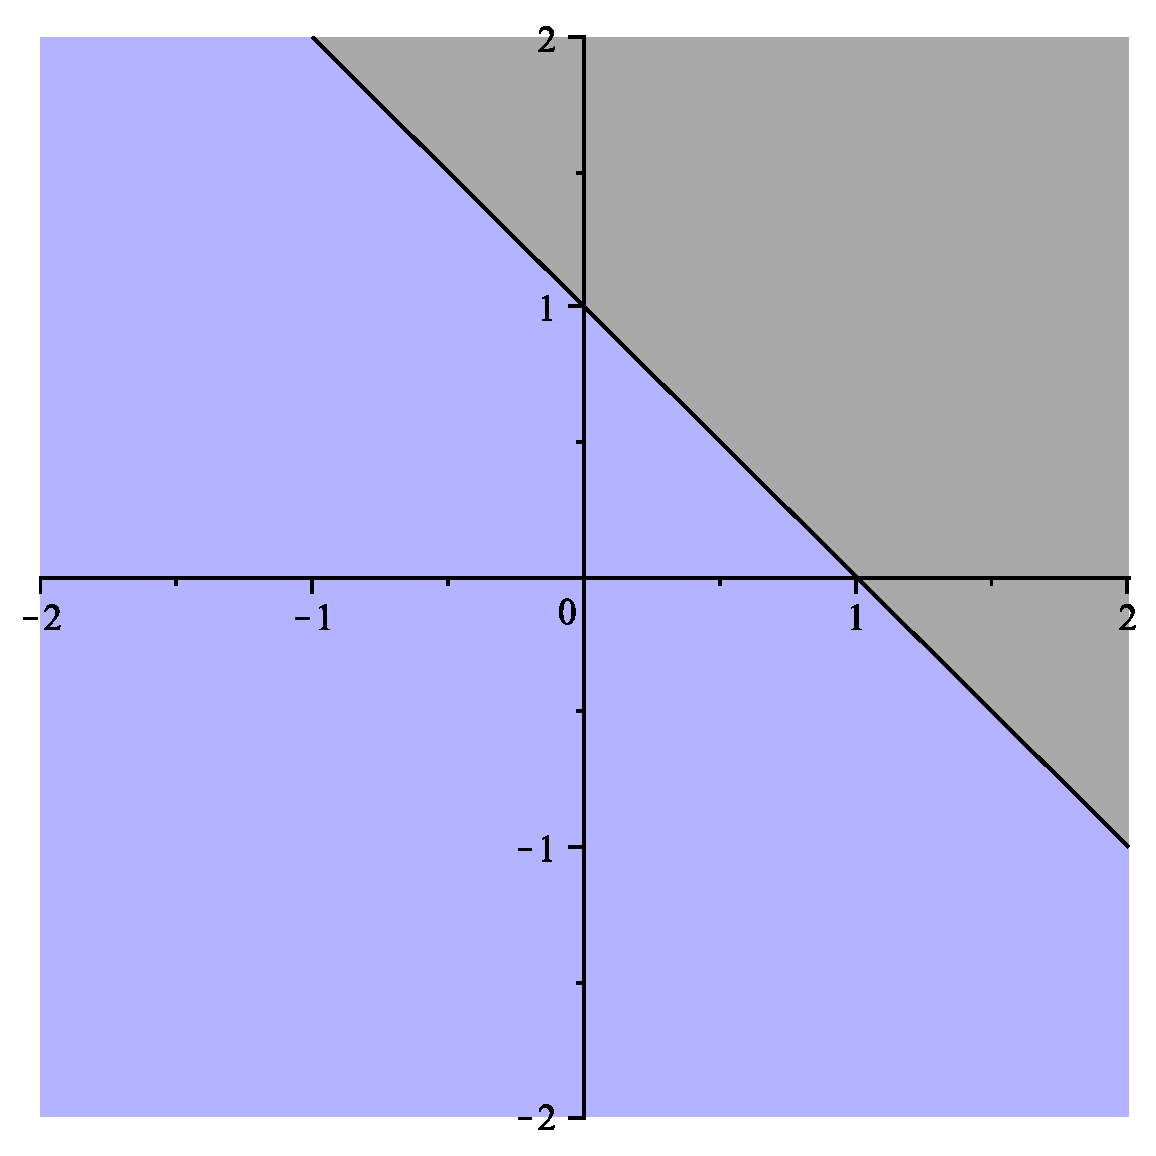
\includegraphics[scale=0.25]{Hl.pdf}}
\subfigure[$H_u$]{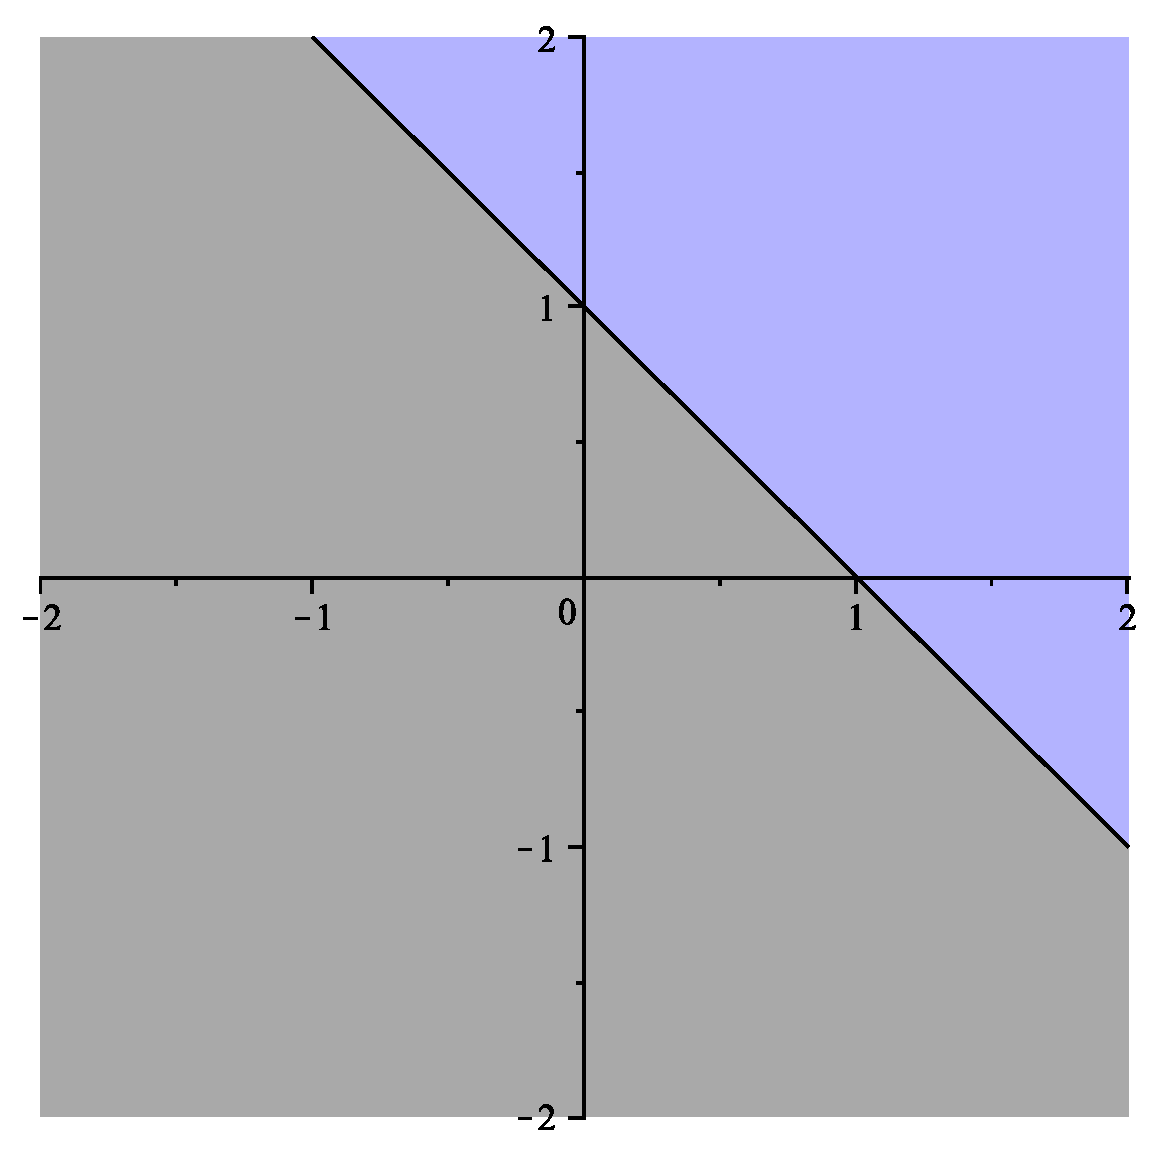
\includegraphics[scale=0.25]{Hu.pdf}}
\caption{Two half-spaces defined by a hyper-plane: A half-space is so named because any hyper-plane divides $\mathbb{R}^n$ (the space in which it resides) into two halves, the side ``on top'' and the side ``on the bottom.''}
\label{fig:HalfSpace}
\end{figure}
A half-space is so named because the hyperplane $\mathbf{a}^T\mathbf{x} = b$ literally separates $\mathbb{R}^n$ into two halves: the half above the hyperplane and the half below the hyperplane.
\end{example}

\begin{lemma} Every hyper-plane is convex.
\end{lemma}
\begin{proof} Let $\mathbf{a} \in \mathbb{R}^n$ and $b \in \mathbb{R}$ and let $H$ be the hyperplane defined by $\mathbf{a}$ and $b$. Choose $\mathbf{x}_1,\mathbf{x}_2 \in{H}$ and $\lambda \in [0,1]$. Let $\mathbf{x} = \lambda\mathbf{x}_1 + (1-\lambda)\mathbf{x}_2$.
By definition we know that:
\begin{gather*}
\mathbf{a}^T\mathbf{x}_1 = b\\
\mathbf{a}^T\mathbf{x}_2 = b
\end{gather*}
Then we have:
\begin{equation}
\mathbf{a}^T\mathbf{x} = \mathbf{a}^T\left[\lambda\mathbf{x}_1 + (1-\lambda)\mathbf{x}_2\right] = 
\lambda\mathbf{a}^T\mathbf{x}_1 + (1-\lambda)\mathbf{a}^T\mathbf{x}_2 = 
\lambda b + (1-\lambda)b = b
\end{equation}
Thus, $\mathbf{x} \in H$ and we see that $H$ is convex. This completes the proof.
\end{proof}
\begin{lemma} Every half-space is convex.
\label{lem:HalfSpaceConvex}
\end{lemma}
\begin{proof}
Let $\mathbf{a} \in \mathbb{R}^n$ and $b \in \mathbb{R}$. Without loss of generality, consider the half-space $H_l$ defined by $\mathbf{a}$ and $b$. For arbitrary $\mathbf{x}_1$ and $\mathbf{x}_2$ in $H_l$ we have:
\begin{gather*}
\mathbf{a}^T\mathbf{x}_1 \leq b\\
\mathbf{a}^T\mathbf{x}_2 \leq b
\end{gather*}
Suppose that $\mathbf{a}^T\mathbf{x}_1 = b_1 \leq b$ and $\mathbf{a}^T\mathbf{x}_2 = b_2 \leq b$. Again let $\mathbf{x} = \lambda\mathbf{x}_1 + (1-\lambda)\mathbf{x}_2$. Then:
\begin{equation}
\mathbf{a}^T\mathbf{x} = \mathbf{a}^T\left[\lambda\mathbf{x}_1 + (1-\lambda)\mathbf{x}_2\right] = 
\lambda\mathbf{a}^T\mathbf{x}_1 + (1-\lambda)\mathbf{a}^T\mathbf{x}_2 = 
\lambda b_1 + (1-\lambda)b_2
\end{equation}
Since $\lambda \leq 1$ and $1-\lambda \leq 1$ and $\lambda \geq 0$ we know that $\lambda b_1 \leq \lambda b$, since $b_1 \leq b$. Similarly we know that $(1-\lambda) b_2 \leq (1-\lambda)b$, since $b_2 \leq b$. Thus:
\begin{equation}
\lambda b_1 + (1-\lambda)b_2 \leq \lambda b + (1-\lambda)b=b
\end{equation}
Thus we have shown that $\mathbf{a}^T\mathbf{x} \leq b$. The case for $H_u$ is identical with the signs of the inequalities reversed. This completes the proof.
\end{proof}

Using these definitions, we are now in a position to define polyhedral sets, which will be the subject of our study for most of the remainder of this chapter. 

\begin{definition}[Polyhedral Set] If $P \subseteq \mathbb{R}^n$ is the intersection of a finite number of half-spaces, then $P$ is a \textit{polyhedral set}. Formally, let $\mathbf{a}_1,\dots,\mathbf{a}_m \in \mathbb{R}^n$ be a finite set of constant vectors and let $b_1,\dots,b_m \in \mathbb{R}$ be constants. Consider the set of half-spaces:
\begin{displaymath}
H_i = \{\mathbf{x} | \mathbf{a}_i^T\mathbf{x} \leq b_i\}
\end{displaymath}
Then the set:
\begin{equation}
P = \bigcap_{i=1}^m H_i
\end{equation}
is a \textit{polyhedral set}.
\label{defn:PolyhedralSet}
\end{definition}

It should be clear that we can represent any polyhedral set using a matrix inequality. The set $P$ is defined by the set of vectors $\mathbf{x}$ satisfying:
\begin{equation}
\mathbf{A}\mathbf{x} \leq \mathbf{b},
\end{equation}
where the \textit{rows} of $\mathbf{A} \in \mathbb{R}^{m \times n}$ are made up of the vectors $\mathbf{a}_1,\dots,\mathbf{a}_m$ and $\mathbf{b} \in \mathbb{R}^m$ is a column vector composed of elements $b_1,\dots,b_m$. 

\begin{theorem} Every polyhedral set is convex.
\label{thm:PolyhedralConvex}
\end{theorem}
\begin{exercise} Prove Theorem \ref{thm:PolyhedralConvex}. [Hint: You can prove this by brute force, verifying convexity. You can also be clever and use two results that we've proved in the notes.]
\end{exercise}

\section{Rays and Directions}
Recall the definition of a \textit{line} (Definition \ref{def:Line} from Chapter 1. A ray is a one sided line. 

\begin{definition}[Ray] Let $\mathbf{x}_0 \in \mathbb{R}^n$ be a point and and let $\mathbf{d} \in \mathbb{R}^n$ be a vector called the \textit{direction}. Then the \textit{ray} with vertex $\mathbf{x}_0$ and direction $\mathbf{d}$ is the collection of points $\{\mathbf{x} | \mathbf{x} = \mathbf{x}_0 + \lambda \mathbf{d},\;\lambda \geq 0\}$.
\end{definition}

\begin{example} We will use the same point and direction as we did for a line in Chapter 1. Let $\mathbf{x_0} = [2,1]^T$ and let $\mathbf{d} = [2,2]^T$. Then the ray defined by $\mathbf{x}_0$ and $\mathbf{d}$ is shown in Figure \ref{fig:LineExample}. The set of points is $R = \{(x,y) \in \mathbb{R}^2 : x = 2 + 2\lambda, y = 1 + 2\lambda, \lambda \geq 0\}$. 
\begin{figure}[ht]
\centering
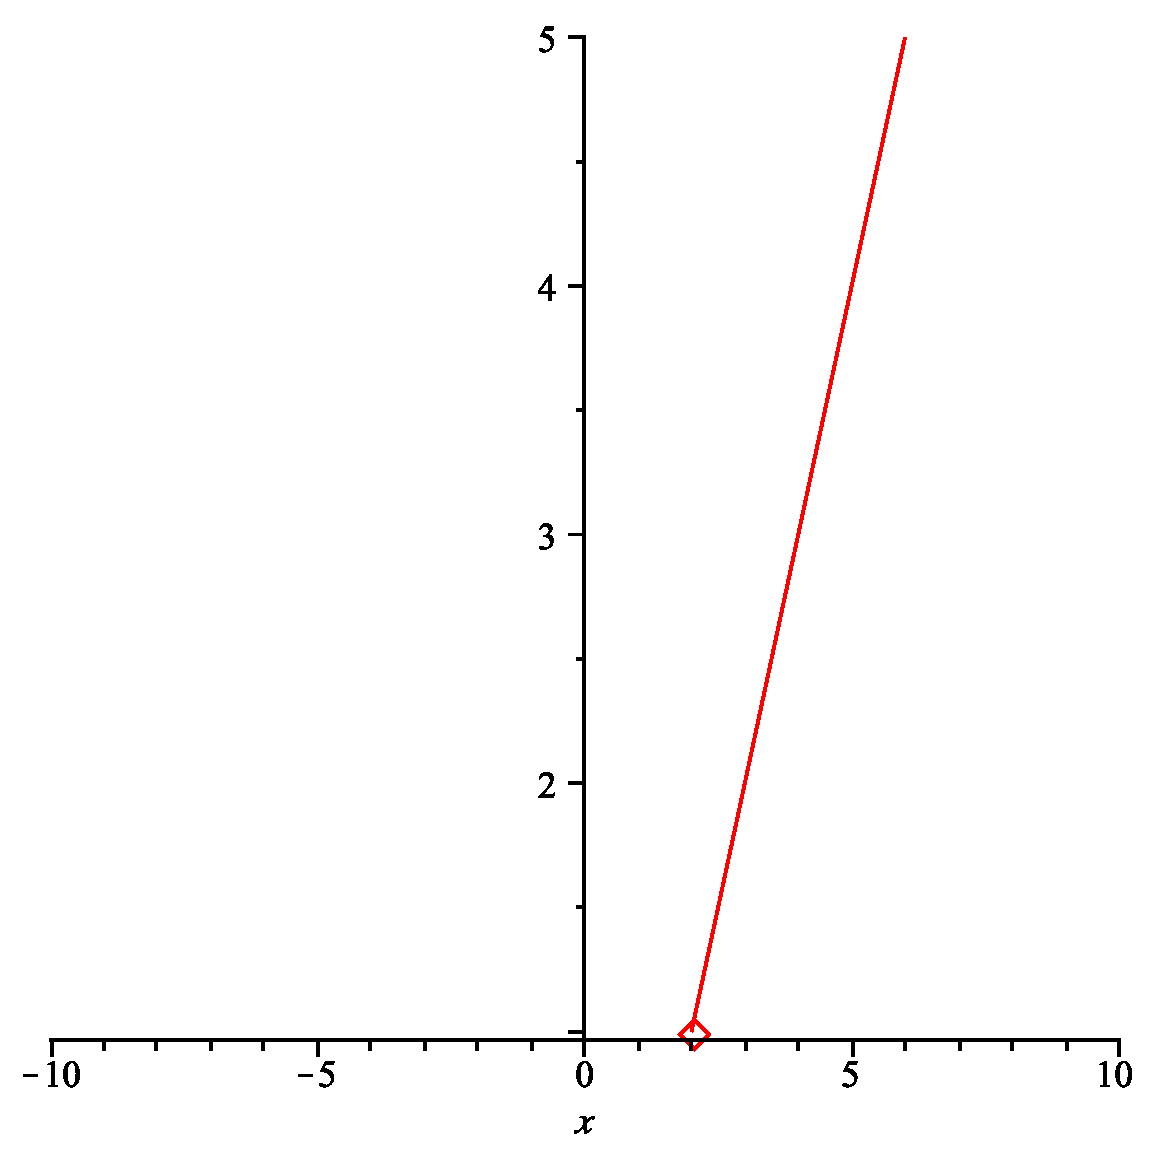
\includegraphics[scale=0.25]{Ray.pdf}
\caption{A Ray: The points in the graph shown in this figure are in the set produced using the expression $\mathbf{x}_0 + \mathbf{d}\lambda$ where $\mathbf{x_0} = [2,1]^T$ and $\mathbf{d} = [2,2]^T$ and $\lambda \geq 0$.}
\label{fig:RayExample}
\end{figure}
\label{ex:BasicRay}
\end{example}

Rays are critical for understanding unbounded convex sets. Specifically, a set is unbounded, in a sense, only if you can show that it contains a ray. An interesting class of unbounded convex sets are convex cones:

\begin{definition}[Convex Cone] Let $C \subseteq \mathbb{R}^n$ be a convex set. Then $C$ is a \textit{convex cone} if for all $\mathbf{x} \in C$ and for all $\lambda \in \mathbb{R}$ with $\lambda \geq 0$ we have $\lambda \mathbf{x} \in C$.
\end{definition}

\begin{lemma} Every convex cone contains the origin.
\label{lem:ConvexConeOrigin}
\end{lemma}

\begin{exercise} Prove the previous lemma. 
\end{exercise}

The fact that every convex cone contains the origin by Lemma \ref{lem:ConvexConeOrigin} along with the fact that for every point $\mathbf{x} \in C$ we have $\lambda\mathbf{x} \in C$ ($\lambda \geq 0$) implies that the ray $\mathbf{0} + \lambda\mathbf{x} \subseteq C$. Thus, since every point $\mathbf{x} \in C$ must be on a ray, it follows that a convex cone is just made up of rays beginning at the origin. 

Another key element to understanding unbounded convex sets is the notion of direction. A direction can be thought of as  a ``direction of travel'' from a starting point inside an unbounded convex set so that you (the traveler) can continue moving forever and never leave the set.

\begin{definition}[Direction of a Convex Set] Let $C$ be a convex set. Then $\mathbf{d}\neq \mathbf{0}$ is a \textit{(recession) direction of the convex set} if for all $\mathbf{x}_0 \in {C}$ the ray with vertex $\mathbf{x}_0$ and direction $\mathbf{d}$ is contained entirely in $C$. Formally, for all $\mathbf{x}_0 \in C$ we have:
\begin{equation}
\left\{\mathbf{x} : \mathbf{x} = \mathbf{x}_0 + \lambda\mathbf{d},\;\lambda \geq 0\right\} \subseteq C
\end{equation}
\end{definition}
\begin{example} Consider the unbounded convex set shown in Figure \ref{fig:ConvexDirectionExample}. This set has direction $[1,0]^T$. 
\begin{figure}[ht]
\centering
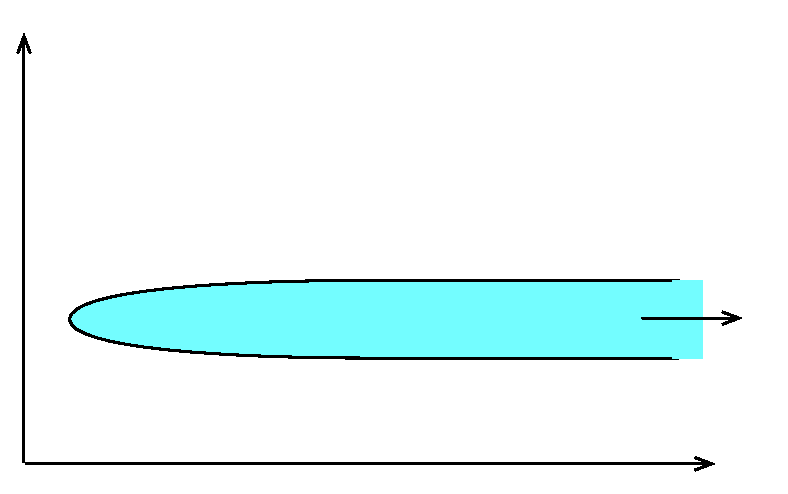
\includegraphics[scale=0.5]{ConvexDirection.pdf}
\caption{Convex Direction: Clearly every point in the convex set (shown in blue) can be the vertex for a ray with direction $[1,0]^T$ contained entirely in the convex set. Thus $[1,0]^T$ is a direction of this convex set.}
\label{fig:ConvexDirectionExample}
\end{figure}
To see this note that for any positive scaling parameter $\lambda$ and for any vertex point $\mathbf{x}_0$, we can draw an arrow pointing to the right (in the direction of $[1,0]^T$) with vertex at $\mathbf{x}_0$ scaled by $\lambda$ that is entirely contained in the convex set.
\end{example}

\begin{exercise} Prove the following: Let $C \subseteq \mathbb{R}^n$ be a convex cone and let $\mathbf{x}_1,\mathbf{x}_2 \in C$. If $\alpha, \beta \in \mathbb{R}$ and $\alpha,\beta \geq 0$, then $\alpha\mathbf{x}_1 + \beta\mathbf{x}_2 \in C$. [Hint: Use the definition of convex cone and the definition of convexity with $\lambda = 1/2$, then multiply by 2.] 
\label{exer:ConvexCone1}
\end{exercise}

\begin{exercise} Use Exercise \ref{exer:ConvexCone1} to prove that if $C \subseteq \mathbb{R}^n$ is a convex cone, then every element $\mathbf{x} \in C$ (except the origin) is also a direction of $C$.
\end{exercise}

\section{Directions of Polyhedral Sets}
There is a unique relationship between the defining matrix $\mathbf{A}$ of a polyhedral set $P$ and a direction of this set that is particularly useful when we assume that $P$ is located in the positive orthant of $\mathbb{R}^n$ (i.e., $\mathbf{x} \geq 0$ are defining constraints of $P$). 
\begin{theorem} Suppose that $P \subseteq \mathbb{R}^n$ is a polyhedral set defined by:
\begin{equation}
P = \left\{\mathbf{x} \in \mathbb{R}^n : \mathbf{A} \mathbf{x} \leq \mathbf{b},\;\mathbf{x} \geq \mathbf{0}\right\}
\end{equation}
If $\mathbf{d}$ is a direction of $P$, then the following hold:
\begin{equation}
\mathbf{A}\mathbf{d} \leq \mathbf{0},\:\mathbf{d} \geq \mathbf{0},\;\mathbf{d} \neq \mathbf{0}. 
\end{equation}
\label{thm:DirectionChar}
\end{theorem}
\begin{proof} The fact that $\mathbf{d} \neq \mathbf{0}$ is clear from the definition of direction of a convex set. Furthermore, $\mathbf{d}$ is a direction if and only if 
\begin{gather}
\mathbf{A}\left(\mathbf{x} + \lambda\mathbf{d}\right) \leq \mathbf{b}\\
\mathbf{x} + \lambda\mathbf{d} \geq \mathbf{0}
\end{gather}
for all $\lambda > 0$ and for all $\mathbf{x} \in P$ (which is to say $\mathbf{x}\in \mathbb{R}^n$ such that $\mathbf{A}\mathbf{x} \leq \mathbf{b}$ and $\mathbf{x} \geq \mathbf{0}$). But then 
\begin{displaymath}
\mathbf{A}\mathbf{x} + \lambda\mathbf{A}\mathbf{d} \leq \mathbf{b}
\end{displaymath}
for all $\lambda > 0$. This can only be true if $\mathbf{A}\mathbf{d} \leq \mathbf{0}$. Likewise:$\mathbf{x} + \lambda\mathbf{d} \geq \mathbf{0}$ holds for all $\lambda > 0$ if and only if $\mathbf{d} \geq \mathbf{0}$. This completes the proof.
\end{proof}
\begin{corollary} If 
\begin{equation}
P = \left\{\mathbf{x} \in \mathbb{R}^n : \mathbf{A} \mathbf{x} = \mathbf{b},\;\mathbf{x} \geq \mathbf{0}\right\}
\end{equation}
and $\mathbf{d}$ is a direction of $P$, then $\mathbf{d}$ must satisfy:
\begin{equation}
\mathbf{A}\mathbf{d} = \mathbf{0},\:\mathbf{d} \geq \mathbf{0},\;\mathbf{d} \neq \mathbf{0}. 
\end{equation}
\end{corollary}
\begin{exercise} Prove the corollary above.
\end{exercise}

\begin{example} Consider the polyhedral set defined by the equations:
\begin{gather*}
x_1 - x_2 \leq 1\\
2x_1 + x_2 \geq 6\\
x_1 \geq 0\\
x_2 \geq 0
\end{gather*}
This set is clearly unbounded as we showed in class and it has at least one direction. The direction $\mathbf{d} = [0,1]^T$ pointing directly up is a direction of this set. This is illustrated in Figure \ref{fig:UnboundedPolyhedron}.
\begin{figure}[htbp]
\centering
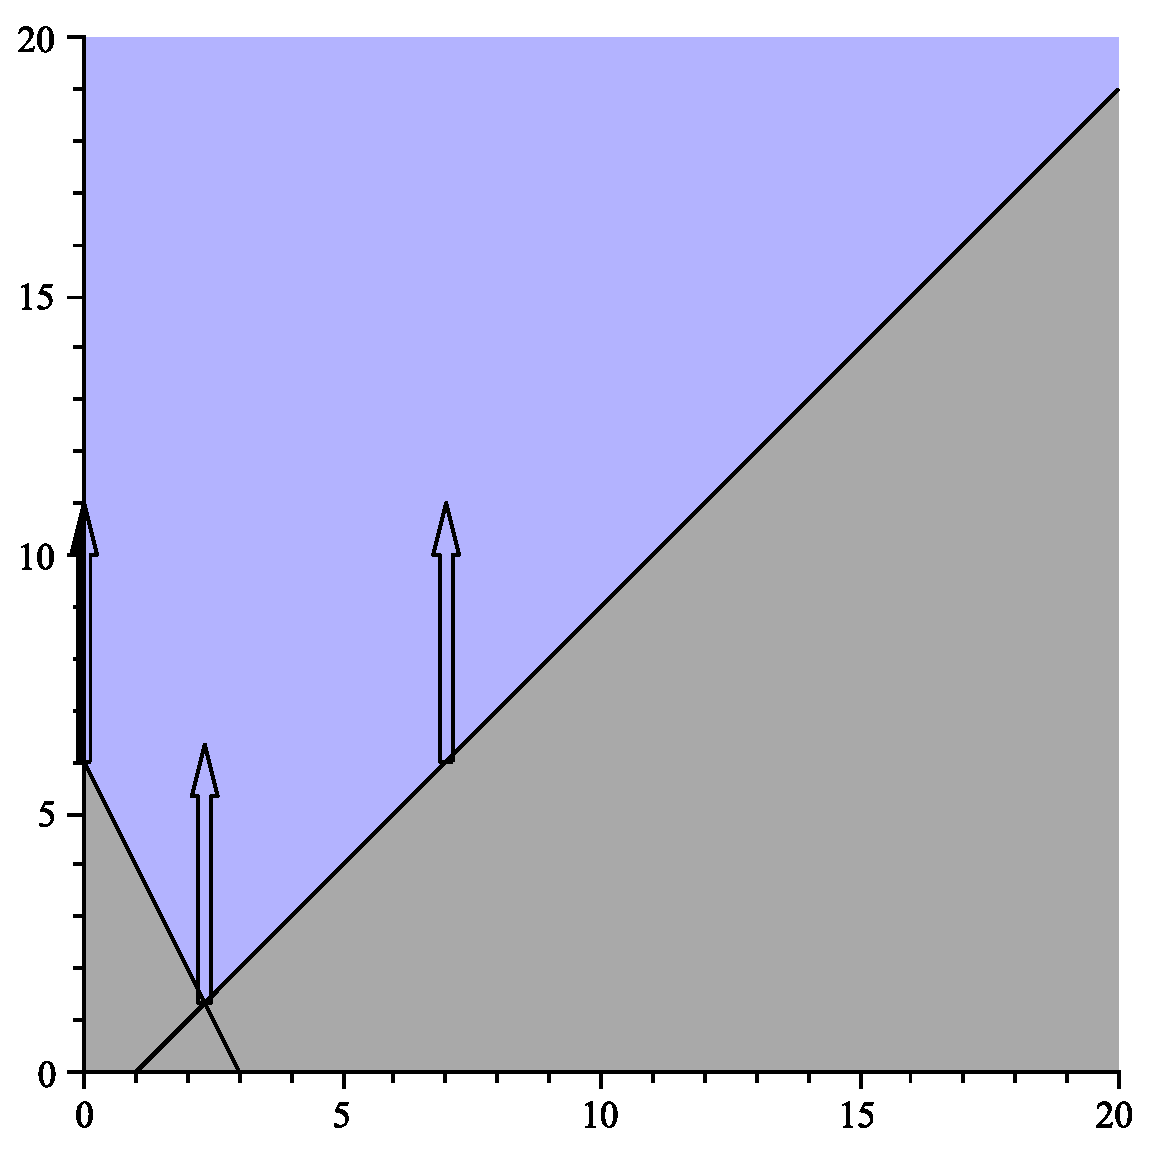
\includegraphics[scale=0.35]{UnboundedPolyhedron.pdf}
\caption{An Unbounded Polyhedral Set: This unbounded polyhedral set has many directions. One direction is $[0,1]^T$.}
\label{fig:UnboundedPolyhedron}
\end{figure}
In this example, we have:
\begin{equation}
\mathbf{A} = \begin{bmatrix}
1 & -1\\
-2 & -1
\end{bmatrix}
\end{equation}
Note, the second inequality constraint was a greater-than constraint. We reversed it to a less-than inequality constraint $-2x_1 - x_2 \leq -6$ by multiplying by $-1$. For our chosen direction $\mathbf{d} = [0,1]^T$, we can see that:
\begin{equation}
\mathbf{A}\mathbf{d} = 
\begin{bmatrix}
1 & -1\\
-2 & -1
\end{bmatrix}
\begin{bmatrix}
0\\
1
\end{bmatrix} = 
\begin{bmatrix}
-1\\
-1
\end{bmatrix} \leq \mathbf{0}
\end{equation}
Clearly $\mathbf{d} \geq \mathbf{0}$ and $\mathbf{d} \neq \mathbf{0}$.
\label{ex:UnboundedPolyhedron}
\end{example}

\section{Extreme Points}
\begin{definition}[Extreme Point of a Convex Set] Let $C$ be a convex set. A point $\mathbf{x}_0 \in C$ is a \textit{extreme point} of $C$ if there are \textit{no points} $\mathbf{x}_1$ and $\mathbf{x}_2$ ($\mathbf{x}_1 \neq \mathbf{x}_0$ or $\mathbf{x}_2 \neq \mathbf{x}_0$) so that
$\mathbf{x} = \lambda\mathbf{x}_1 + (1-\lambda)\mathbf{x}_2$ for some $\lambda \in (0,1)$.\footnote{Thanks to Bob Pakzad-Hurson who fixed a typo in this definition in Version $\leq$ 1.4.}
\label{defn:ExtremePoint}
\end{definition}

An extreme point is simply a point in a convex set $C$ that cannot be expressed as a strict convex combination of any other pair of points in $C$. We will see that extreme points must be located in specific locations in convex sets. 

\begin{definition}[Boundary of a set] Let $C \subseteq \mathbb{R}^n$ be (convex) set. A point $\mathbf{x}_0 \in C$ is on the \textit{boundary} of $C$ if for all $\epsilon > 0$, 
\begin{gather*}
B_\epsilon(\mathbf{x}_0) \cap C \neq \emptyset \;\text{and}\\
B_\epsilon(\mathbf{x}_0) \cap \mathbb{R}^n \setminus C \neq \emptyset
\end{gather*}
\end{definition}
\begin{example} A convex set, its boundary and a boundary point are illustrated in Figure \ref{fig:BoundaryPoint}.
\begin{figure}[htbp]
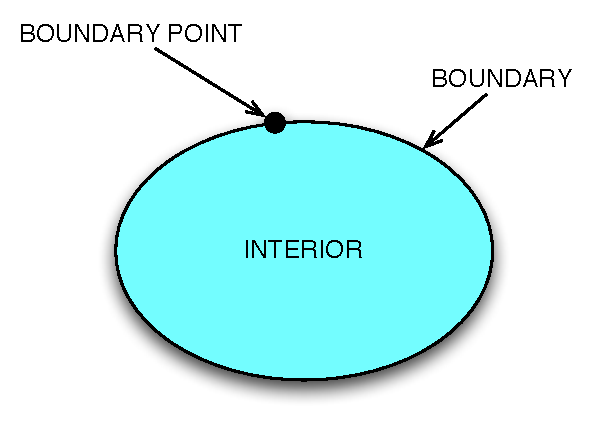
\includegraphics[scale=0.5]{Boundary.pdf}
\caption{Boundary Point: A boundary point of a (convex) set $C$ is a point in the set so that for \textit{every} ball of any radius centered at the point contains some points inside $C$ and some points outside $C$.}
\label{fig:BoundaryPoint}
\end{figure}
\end{example}

\begin{lemma} Suppose $C$ is a convex set. If $\mathbf{x}$ is an extreme point of $C$, then $\mathbf{x}$ is on the boundary of $C$. 
\label{lem:BoundaryExtremePoint}
\end{lemma}
\begin{proof} Suppose not, then $\mathbf{x}$ is not on the boundary and thus there is some $\epsilon > 0$ so that $B_\epsilon(\mathbf{x}_0) \subset C$. Since $B_\epsilon(\mathbf{x}_0)$ is a hypersphere, we can choose two points $\mathbf{x}_1$ and $\mathbf{x}_2$ on the boundary of $B_\epsilon(\mathbf{x}_0)$ so that the line segment between these points passes through the center of $B_\epsilon(\mathbf{x}_0)$. But this center point is $\mathbf{x}_0$. Therefore $\mathbf{x}_0$ is the mid-point of $\mathbf{x}_1$ and $\mathbf{x}_2$ and since $\mathbf{x}_1,\mathbf{x}_2 \in C$ and $\lambda\mathbf{x}_1 + (1-\lambda)\mathbf{x}_2 = \mathbf{x}_0$ with $\lambda = 1/2$ it follows that $\mathbf{x}_0$ cannot be an extreme point, since it is a strict convex combination of $\mathbf{x}_1$ and $\mathbf{x}_2$. This completes the proof.
\end{proof}

Most important in our discussion of linear programming will be the extreme points of polyhedral sets that appear in linear programming problems. The following theorem establishes the relationship between extreme points in a polyhedral set and the intersection of hyperplanes in such a set.

\begin{theorem} Let $P \subseteq \mathbb{R}^n$ be a polyhedral set and suppose $P$ is defined as:
\begin{equation}
P = \{\mathbf{x} \in \mathbb{R}^n : \mathbf{A}\mathbf{x} \leq \mathbf{b}\}
\end{equation}
where $\mathbf{A} \in \mathbb{R}^{m \times n}$ and $\mathbf{b} \in \mathbb{R}^m$. A point $\mathbf{x}_0 \in P$ is an extreme point of $P$ if and only if $\mathbf{x}_0$ is the intersection of $n$ linearly independent hyperplanes from the set defining $P$. 
\label{thm:DefExtremePoint}
\end{theorem}

\begin{remark}The easiest way to see this as relevant to linear programming is to assume that 
\begin{equation}
P = \{\mathbf{x} \in \mathbb{R}^n : \mathbf{A}\mathbf{x} \leq \mathbf{b},\;\mathbf{x} \geq \mathbf{0}\}
\end{equation}
In this case, we could have $m < n$. In that case, $P$ is composed of the intersection of $n + m$ half-spaces. The first $m$ are for the rows of $\mathbf{A}$ and the second $n$ are for the non-negativity constraints. An extreme point comes from the intersection of $n$ of the hyperplanes defining these half-spaces. We  might have $m$ come from the constraints $\mathbf{A}\mathbf{x} \leq \mathbf{b}$ and the other $n-m$ from $\mathbf{x} \geq \mathbf{0}$.
\end{remark}

\begin{proof}
($\Leftarrow$) Suppose that $\mathbf{x}_0$ is the intersection of $n$ hyperplanes. Then $\mathbf{x}_0$ lies on $n$ hyperplanes. By way of contradiction of suppose that $\mathbf{x}_0$ is not an extreme point. Then there are two points $\overline{\mathbf{x}}, \hat{\mathbf{x}} \in P$ and a scalar $\lambda \in (0,1)$ so that
\begin{displaymath}
\mathbf{x}_0 = \lambda\overline{\mathbf{x}} + (1-\lambda)\hat{\mathbf{x}}
\end{displaymath}
If this is true, then for some $\mathbf{G} \in \mathbb{R}^{n\times n}$ whose rows are drawn from $\mathbf{A}$ and a vector $\mathbf{g}$ whose entries are drawn from the vector $\mathbf{b}$, so that $\mathbf{G}\mathbf{x}_0 = \mathbf{g}$. But then we have:
\begin{equation}
\mathbf{g} = \mathbf{G}\mathbf{x}_0 = \lambda\mathbf{G}\overline{\mathbf{x}} + (1-\lambda)\mathbf{G}\hat{\mathbf{x}}
\label{eqn:gequal}
\end{equation}  
and $\mathbf{G}\overline{\mathbf{x}} \leq \mathbf{g}$ and $\mathbf{G}\hat{\mathbf{x}}\leq \mathbf{g}$ (since $\overline{\mathbf{x}}, \hat{\mathbf{x}} \in P$). But the only way for Equation \ref{eqn:gequal} to hold is if 
\begin{enumerate*}
\item $\mathbf{G}\overline{\mathbf{x}} = \mathbf{g}$ and
\item $\mathbf{G}\hat{\mathbf{x}} = \mathbf{g}$
\end{enumerate*}
The fact that the hyper-planes defining $\mathbf{x}_0$ are linearly independent implies that the solution to $\mathbf{G}\mathbf{x}_0 = \mathbf{g}$ is unique. (That is, we have chosen $n$ equations in $n$ unknowns and $\mathbf{x}_0$ is the solution to these $n$ equations.) Therefore, it follows that $\mathbf{x}_0 = \overline{\mathbf{x}}=\hat{\mathbf{x}}$ and thus $\mathbf{x}_0$ is an extreme point since it cannot be expressed as a convex combination of other points in $P$.

($\Rightarrow$) By Lemma \ref{lem:BoundaryExtremePoint}, we know that any extreme point $\mathbf{x}_0$ lies on the boundary of $P$ and therefore there is at least one row $\mathbf{A}_{i\cdot}$ such that $\mathbf{A}_{i\cdot}\mathbf{x}_0 = \mathbf{b}_i$ (otherwise, clearly $\mathbf{x}_0$ does not lie on the boundary of $P$). By way of contradiction, suppose that $\mathbf{x}_0$ is the intersection of $r < n$ linearly independent hyperplanes (that is, only these $r$ constraints are binding). Then there is a matrix $\mathbf{G} \in \mathbb{R}^{r \times n}$ whose rows are drawn from $\mathbf{A}$ and a vector $\mathbf{g}$ whose entries are drawn from the vector $\mathbf{b}$, so that $\mathbf{G}\mathbf{x}_0 = \mathbf{g}$. Linear independence of the hyperplanes implies that the rows of $\mathbf{G}$ are linearly independent and therefore there is a non-zero solution to the equation $\mathbf{G}\mathbf{d} = \mathbf{0}$. To see this, apply Expression \ref{eqn:BasicVars} and choose solution in which $\mathbf{d}$ is non-zero. Then we can find an $\epsilon > 0$ such that:
\begin{enumerate*}
\item If $\overline{\mathbf{x}} = \mathbf{x}_0 + \epsilon\mathbf{d}$, then $\mathbf{G}\overline{\mathbf{x}} = \mathbf{g}$ \textit{and} all non-binding constraints at $\mathbf{x}_0$ remain non-binding at $\overline{\mathbf{x}}$.

\item If $\hat{\mathbf{x}} = \mathbf{x}_0 - \epsilon\mathbf{d}$, then $\mathbf{G}\hat{\mathbf{x}} = \mathbf{g}$ \textit{and} all non-binding constraints at $\mathbf{x}_0$ remain non-binding at $\hat{\mathbf{x}}$.
\end{enumerate*}
These two facts hold since $\mathbf{G}\mathbf{d} = \mathbf{0}$ and if $\mathbf{A}_{i\cdot}$ is a row of $\mathbf{A}$ with $\mathbf{A}_{i\cdot}\mathbf{x}_0 < \mathbf{b}_i$ (or $\mathbf{x} > 0$), then there is at least one non-zero $\epsilon$ so that $\mathbf{A}_{i\cdot}(\mathbf{x}_0 \pm \epsilon \mathbf{d}) < \mathbf{b}_i$ (or $\mathbf{x}_0 \pm \epsilon \mathbf{d} > \mathbf{0}$) still holds and therefore $(\mathbf{x}_0 \pm \epsilon \mathbf{d}) \in P$. Since we have a finite number of constraints that are non-binding, we may choose $\epsilon$ to be the smallest value so that the previous statements hold for all of them. Finally we can choose $\lambda = 1/2$ and see that $\mathbf{x}_0 = \lambda\overline{\mathbf{x}} + (1-\lambda)\hat{\mathbf{x}}$ and $\overline{\mathbf{x}}, \hat{\mathbf{x}} \in P$. Thus $\mathbf{x}_0$ cannot have been an extreme point, contradicting our assumption. This completes the proof.
\end{proof}

\begin{definition} Let $P$ be the polyhedral set from Theorem \ref{thm:DefExtremePoint}. If $\mathbf{x}_0$ is an extreme point of $P$ and \textit{more} than $n$ hyperplanes are binding at $\mathbf{x}_0$, then $\mathbf{x}_0$ is called a \textit{degenerate} extreme point.
\end{definition}

\begin{definition}[Face] Let $P$ be a polyhedral set defined by
\begin{displaymath}
P = \{\mathbf{x} \in \mathbb{R}^n : \mathbf{A}\mathbf{x} \leq \mathbf{b}\}
\end{displaymath}
where $\mathbf{A} \in \mathbb{R}^{m\times n}$ and $\mathbf{b} \in \mathbb{R}^m$. If $X \subseteq P$ is defined by a non-empty set of binding linearly independent hyperplanes, then $X$ is a \textit{face} of $P$. 

That is, there is some set of linearly independent rows $A_{i_1\cdot},\dots A_{i_l\cdot}$ with $i_l < m$ so that when $\mathbf{G}$ is the matrix made of these rows and $\mathbf{g}$ is the vector of $b_{i_1},\dots,b_{i_l}$ then: 
\begin{equation}
X = \{\mathbf{x} \in \mathbb{R}^n : \mathbf{G}\mathbf{x} = \mathbf{g} \text{ and } \mathbf{A}\mathbf{x} \leq \mathbf{b}\}
\end{equation}
In this case we say that $X$ has \textit{dimension} $n - l$. 
\end{definition}

\begin{remark} Based on this definition, we can easily see that an extreme point, which is the intersection $n$ linearly independent hyperplanes is a face of dimension zero. 
\end{remark}

\begin{definition}[Edge and Adjacent Extreme Point] An edge of a polyhedral set $P$ is any face of dimension 1. Two extreme points are called \textit{adjacent} if they share $n-1$ binding constraints. That is, they are connected by an edge of $P$.
\end{definition} 

\begin{example} Consider the polyhedral set defined by the system of inequalities:
\begin{gather*}
3x_1 + x_2 \leq 120\\
x_1 + 2x_2 \leq 160\\
\frac{28}{16}x_1+x_2 \leq 100\\
x_1 \leq 35\\
x_1 \geq 0\\
x_2 \geq 0
\end{gather*}
The polyhedral set is shown in Figure \ref{fig:PolyhedralSet}.
\begin{figure}[htbp]
\centering
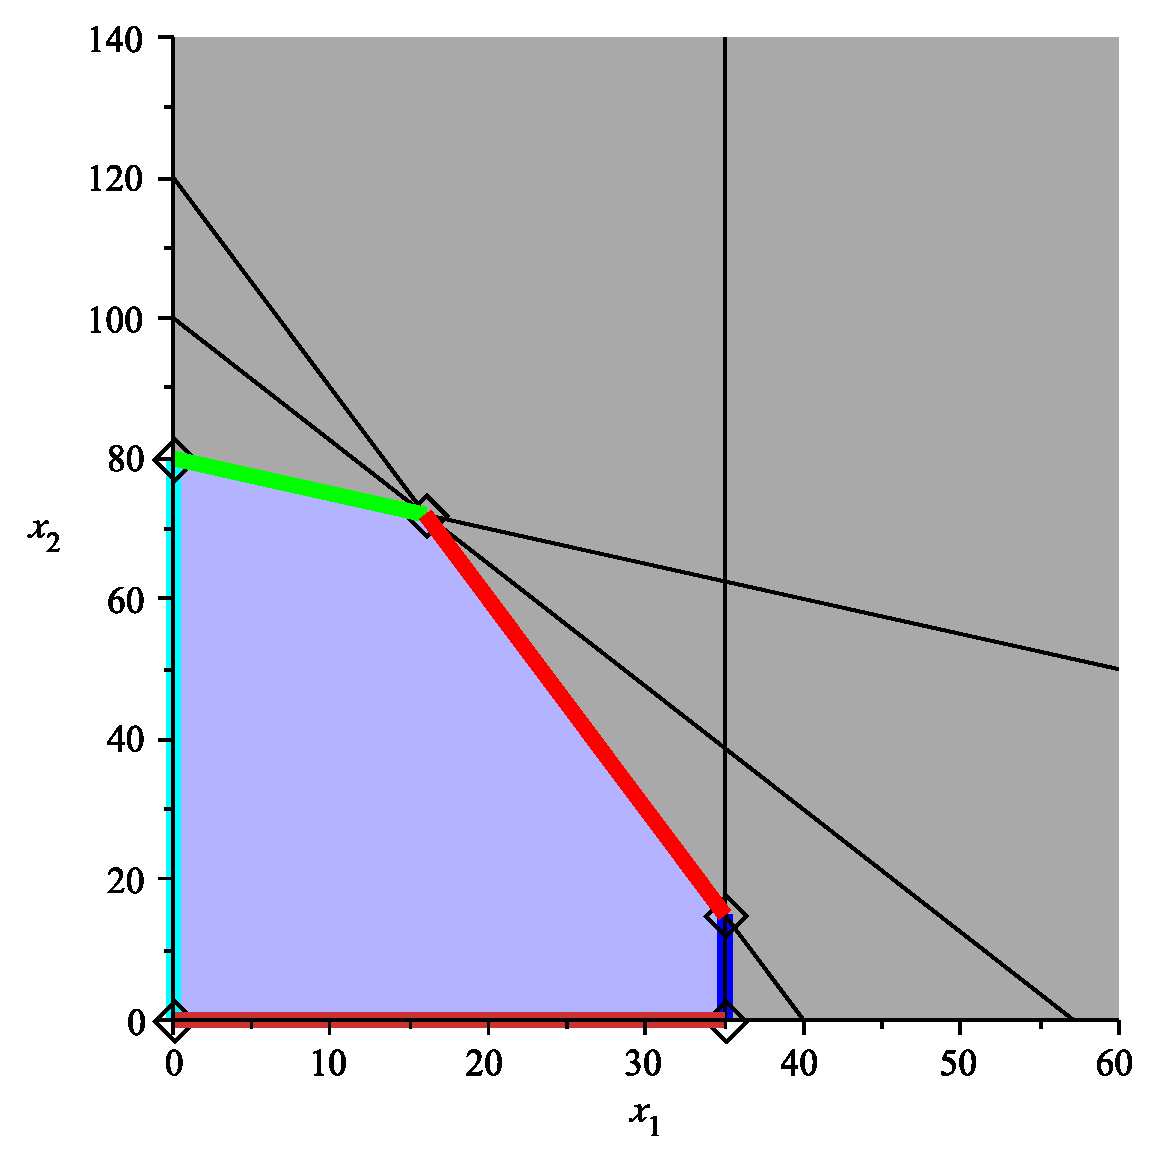
\includegraphics[scale=0.35]{PolyhedronExample.pdf}
\caption{A Polyhedral Set: This polyhedral set is defined by five half-spaces and has a single degenerate extreme point located at the intersection of the binding constraints $3x_1 + x_2 \leq 120$, $x_1 + 2x_2 \leq 160$ and $\frac{28}{16}x_1+x_2 <= 100$. All faces are shown in bold.}
\label{fig:PolyhedralSet}
\end{figure}
The extreme points of the polyhedral set are shown as large diamonds and correspond to intersections of binding constraints. Note the extreme point $(16,72)$ is \textit{degenerate} since it occurs at the intersection of three binding constraints $3x_1 + x_2 \leq 120$, $x_1 + 2x_2 \leq 160$ and $\frac{28}{16}x_1+x_2 <= 100$. All the faces of the polyhedral set are shown in bold. They are locations where one constraint (or half-space) is binding. An example of a pair of adjacent extreme points is $(16,72)$ and $(35,15)$, as they are connected by the edge defined by the binding constraint $3x_1 + x_2 \leq 120$.
\label{ex:ToyMakerDegen}
\end{example}

\begin{exercise} Consider the polyhedral set defined by the system of inequalities:
\begin{gather*}
4x_1 + x_2 \leq 120\\
x_1 + 8x_2 \leq 160\\
x_1 + x_2 \leq 30\\
x_1 \geq 0\\
x_2 \geq 0
\end{gather*}
Identify all extreme points and edges in this polyhedral set and their binding constraints. Are any extreme points degenerate? List all pairs of adjacent extreme points.
\end{exercise}

\section{Extreme Directions}
\begin{definition}[Extreme Direction] Let $C \subseteq\mathbb{R}^n$ be a convex set. Then a direction $\mathbf{d}$ of $C$ is an \textit{extreme direction} if there are no two other directions $\mathbf{d}_1$ and $\mathbf{d}_2$ of $C$ ($\mathbf{d}_1 \neq \mathbf{d}$ and $\mathbf{d}_2 \neq \mathbf{d}$) and scalars $\lambda_1,\lambda_2 > 0$ so that $\mathbf{d} = \lambda_1\mathbf{d}_1 + \lambda_2\mathbf{d}_2$. 
\end{definition}

We have already seen by Theorem \ref{thm:DirectionChar} that is $P$ is a polyhedral set in the positive orthant of $\mathbb{R}^n$ with form:
\begin{displaymath}
P = \left\{\mathbf{x} \in \mathbb{R}^n : \mathbf{A} \mathbf{x} \leq \mathbf{b},\;\mathbf{x} \geq \mathbf{0}\right\}
\end{displaymath}
then a direction $\mathbf{d}$ of $P$ is characterized by the set of inequalities and equations
\begin{displaymath}
\mathbf{A}\mathbf{d} \leq \mathbf{0},\:\mathbf{d} \geq \mathbf{0},\;\mathbf{d} \neq \mathbf{0}.
\end{displaymath}
Clearly two directions $\mathbf{d}_1$ and $\mathbf{d}_2$ with $\mathbf{d_1} = \lambda\mathbf{d}_2$ for some $\lambda \geq 0$ may both satisfy this system. To isolate a unique set of directions, we can normalize and construct the set:
\begin{equation}
D = \{\mathbf{d} \in \mathbb{R}^n : \mathbf{A}\mathbf{d} \leq \mathbf{0},\;\mathbf{d} \geq \mathbf{0},\mathbf{e}^T\mathbf{d} = 1\}
\end{equation}
here we are interested only in directions satisfying $\mathbf{e}^T\mathbf{d} = 1$. This is a normalizing constraint that will chose only vectors whose components sum to 1.

\begin{theorem} A direction $\mathbf{d} \in D$ is an extreme direction of $P$ if and only if $\mathbf{d}$ is an extreme point of $D$ when $D$ is taken as a polyhedral set.
\label{thm:ExtremeDirections}
\end{theorem}
\begin{proof} 
($\Rightarrow$)Suppose that $\mathbf{d}$ is an extreme point of $D$ (as a polyhedral set) and not an extreme direction of $P$. Then there exist two directions $\mathbf{d}_1$ and $\mathbf{d}_2$ of $P$ and two constants $\lambda_1$ and $\lambda_2$ with $\lambda_1,\lambda_2 \geq 0$ so that $\mathbf{d} = \lambda_1\mathbf{d}_1 + \lambda_2\mathbf{d}_2$. Without loss of generality, we may assume that $\mathbf{d}_1$ and $\mathbf{d}_2$ are vectors satisying $\mathbf{e}^T\mathbf{d}_i = 1$ ($i=1,2$). If not, then we can scale them so their components sum to 1 and adjust $\lambda_1$ and $\lambda_2$ accordingly. But this implies that:
\begin{displaymath}
1 = \mathbf{e}^T\mathbf{d} = \lambda_1 \mathbf{e}^T\mathbf{d}_1 + \lambda_2\mathbf{e}^T\mathbf{d}_2 = \lambda_1 + \lambda_2
\end{displaymath}
Further, the fact that $\mathbf{d}_1$ and $\mathbf{d}_2$ are directions of $P$ implies they must be in $D$. Thus we have found a convex combination of element of $D$ that equals $\mathbf{d}$, contradicting our assumption that $\mathbf{d}$ was an extreme point.

($\Leftarrow$)Conversely, suppose that $\mathbf{d}$ is an extreme direction  of $P$ whose components sum to 1 and not an extreme point of $D$. (Again, we could scale $\mathbf{d}$ if needed.) Then $\mathbf{d}$ cannot be recovered from a positive combination of directions $\mathbf{d}_1$ and $\mathbf{d}_2$. But if $\mathbf{d}$ is not an extreme point of $D$, then we know $\lambda_1\mathbf{d}_1 + \lambda_2\mathbf{d}_2 = \mathbf{d}$ for $\mathbf{d}_1,\mathbf{d}_2 \in D$ and $\lambda_1 + \lambda_2 = 1$ and $\lambda_1,\lambda_2 \in (0,1)$. This is clearly contradictory. Every strict convex combination is a positive combination and therefore our assumption that $\mathbf{d}$ was an extreme direction was false.
\end{proof}

\begin{example} Let's consider Example \ref{ex:UnboundedPolyhedron} again. The polyhedral set in this example was defined by the $\mathbf{A}$ matrix:
\begin{displaymath}
\mathbf{A} = \begin{bmatrix}
1 & -1\\
-2 & -1
\end{bmatrix}
\end{displaymath} 
and the $\mathbf{b}$ vector:
\begin{displaymath}
\mathbf{b} = \begin{bmatrix}
1 \\
-6
\end{bmatrix}
\end{displaymath}
If we assume that $P = \left\{\mathbf{x} \in \mathbb{R}^n : \mathbf{A} \mathbf{x} \leq \mathbf{b},\;\mathbf{x} \geq 0\right\}$, then the set of extreme directions of $P$ is the same as the set of extreme points of the set 
\begin{displaymath}
D = \{\mathbf{d} \in \mathbb{R}^n : \mathbf{A}\mathbf{d} \leq \mathbf{0},\;\mathbf{d} \geq \mathbf{0},\mathbf{e}^T\mathbf{d} = 1\}
\end{displaymath}
Then we have the set of directions $\mathbf{d} = [d_1,d_2]^T$ so that:
\begin{gather*}
d_1 - d_2 \leq 0\\
-2d_1 - d_2 \leq 0\\
d_1 + d_2 = 1\\
d_1 \geq 0\\
d_2 \geq 0
\end{gather*}
The feasible region (which is really only the line $d_1 + d_2 = 1$) is shown in red in Figure \ref{fig:DExtreme}.
\begin{figure}[htbp]
\centering
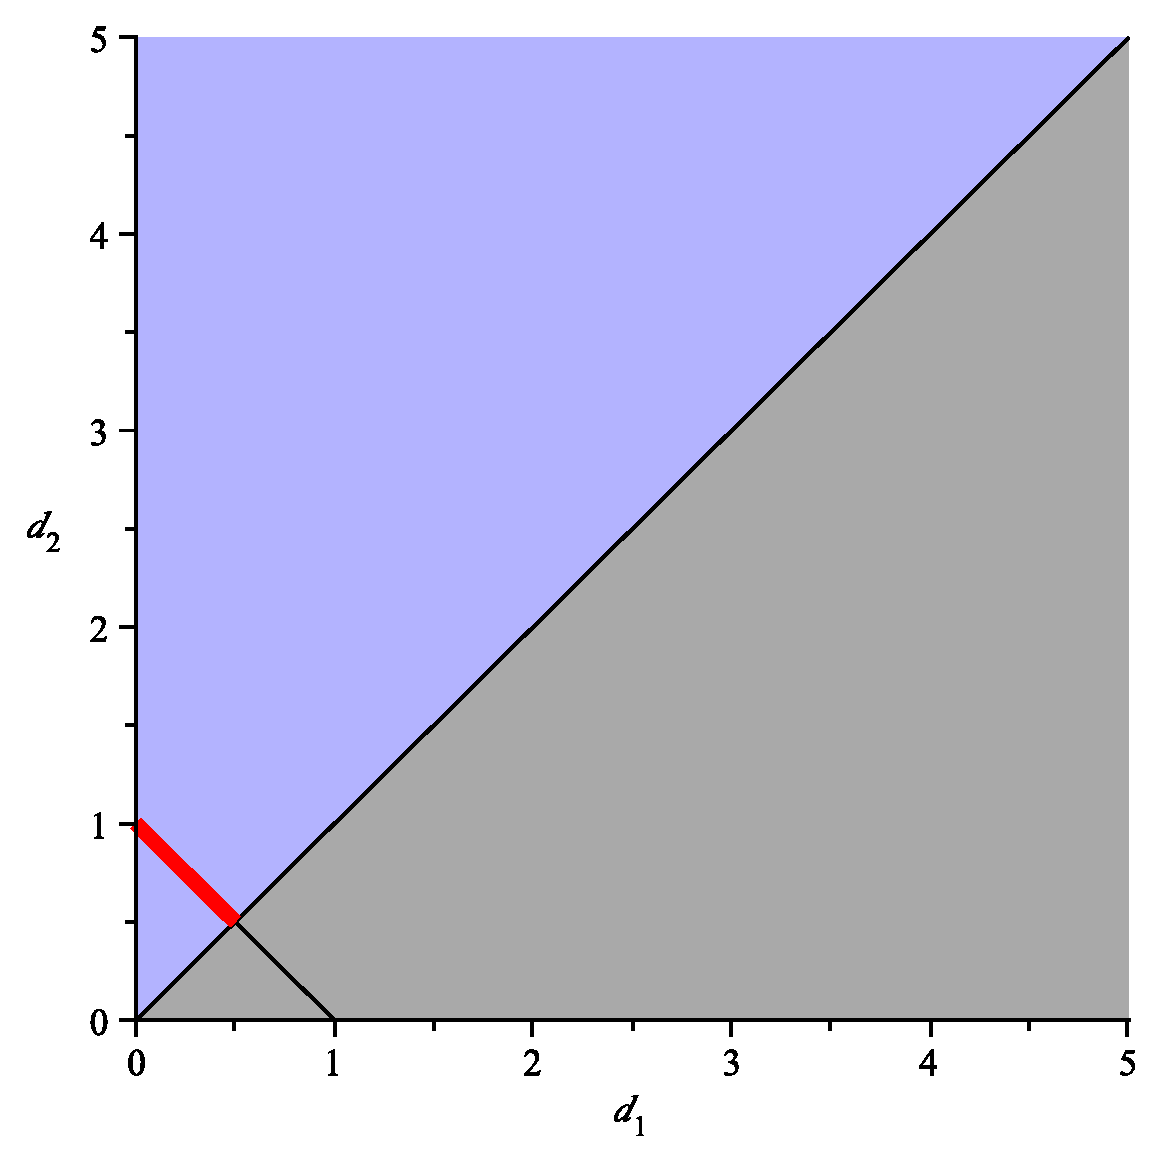
\includegraphics[scale=0.35]{DExtreme.pdf}
\caption{Visualization of the set $D$: This set really consists of the set of points on the red line. This is the line where $d_1 + d_2 = 1$ and all other constraints hold. This line has two extreme points $(0,1)$ and $(1/2,1/2)$.}
\label{fig:DExtreme}
\end{figure}
The critical part of this figure is the red line. It is the true set $D$. As a line, it has two extreme points: $(0,1)$ and $(1/2,1/2)$. Note that $(0,1)$ as an extreme point is one of the direction $[0,1]^T$ we illustrated in Example \ref{ex:UnboundedPolyhedron}.
\end{example}

\begin{exercise} Show that $\mathbf{d} = [1/2,1/2]^T$ is a direction of the polyhedral set $P$ from Example \ref{ex:UnboundedPolyhedron}. Now find a non-extreme direction (whose components sum to $1$) using the feasible region illustrated in the previous example. Show that the direction you found is a direction of the polyhedral set. Create a figure like Figure \ref{fig:UnboundedPolyhedron} to illustrate \textit{both} these directions.
\end{exercise}

\section{Caratheodory Characterization Theorem}
\begin{lemma} The polyhedral set defined by:
\begin{displaymath}
P = \left\{\mathbf{x} \in \mathbb{R}^n : \mathbf{A} \mathbf{x} \leq \mathbf{b},\;\mathbf{x} \geq \mathbf{0}\right\}
\end{displaymath}
has a finite, non-zero number of extreme points (assuming that $\mathbf{A}$ is not an empty matrix)\footnote{Thanks to Bob Pakzah-Hurson for the suggestion to improve the statement of this lemma.}.
\label{lem:FiniteExtremePoints}
\end{lemma}
\begin{proof} 
Let $\mathbf{x} \in P$. If $\mathbf{x}$ is an extreme point, then the theorem is proved. Suppose that $\mathbf{x}$ is not an extreme point. Then by Theorem \ref{thm:DefExtremePoint}, $\mathbf{x}$ lies at the intersection of $r < n$ binding constraints (where $r$ could be zero). The fact that $\mathbf{x}$ is not an extreme point of $P$ implies the existence of $\mathbf{y}_1, \mathbf{y}_2 \in P$ and a $\lambda > 0$ so that $\mathbf{x} = \lambda\mathbf{y}_1 + (1 - \lambda)\mathbf{y}_2$. For this to hold, we know that the $r$ constraints that bind at $\mathbf{x}$ must also be binding at $\mathbf{y}_1$ and $\mathbf{y}_2$.

Let $\mathbf{d} = \mathbf{y}_2 - \mathbf{y}_1$ be the direction from $\mathbf{y}_1$ to $\mathbf{y}_2$. We can see that:
\begin{equation}
\begin{aligned}
\mathbf{y}_1 = &\mathbf{x} - (1-\lambda)\mathbf{d}\\
\mathbf{y}_2 = &\mathbf{x} + \lambda\mathbf{d}
\end{aligned}
\label{eqn:Directions}
\end{equation}
The values $\mathbf{x} + \gamma\mathbf{d}$ and $\mathbf{x} - \gamma\mathbf{d}$ for $\gamma > 0$ correspond to motion from $\mathbf{x}$ along the direction of $\mathbf{d}$. From Expression \ref{eqn:Directions}, we can move in either the positive or negative direction of $\mathbf{d}$ and remain in $P$. Let $\gamma$ be the \textit{largest} value so that both $\mathbf{x} + \gamma\mathbf{d}$ or $\mathbf{x} - \gamma\mathbf{d}$ is in $P$. Clearly we cannot move in both directions infinitely far since $\mathbf{x} \geq \mathbf{0}$ and hence $\gamma < \infty$. Without loss of generality, suppose that $\gamma$ is determined by $\mathbf{x} - \gamma\mathbf{d}$. (That is, $\mathbf{x} - (\gamma + \epsilon)\mathbf{d} \not\in P$ for $\epsilon > 0$). Let $\mathbf{x}_1 = \mathbf{x} - \gamma\mathbf{d}$. Since $r$ hyperplanes are binding at $\mathbf{x}$ (and $\mathbf{y}_1$ and $\mathbf{y}_2)$ it is clear that these same hyperplanes are binding at $\mathbf{x}_1$ and at least one more (because of how we selected $\gamma$). Thus there are at least $r+1$ binding hyperplanes at $\mathbf{x}_1$. If $r+1 = n$, then we have identified an extreme point. Otherwise, we may repeat the process until we find an extreme point. 

To show that the number of extreme points is finite, we note that every extreme point is the intersection of $n$ linearly independent hyperplanes defining $P$. There are $n+m$ hyperplanes defining $P$ and therefore the number of possible extreme points is limited by $\binom{n+m}{n}$. This completes the proof.
\end{proof}

\begin{lemma} Let $P$ be a non-empty polyhedral set. Then the set of directions of $P$ is empty if and only if $P$ is bounded. 
\end{lemma}
\begin{proof} Clearly if $P$ is bounded then it cannot have a direction. If $P$ were contained in a ball $B_r(\mathbf{x}_0)$ then we know that for every $\mathbf{x} \in P$ we have $|\mathbf{x}-\mathbf{x}_0| < r$. If $\mathbf{d}$ is a direction of $P$, then we have $\mathbf{x} + \lambda\mathbf{d}$ for all $\lambda > 0$. We simply need to choose $\lambda$ large enough so that $|\mathbf{x} + \lambda\mathbf{d}-\mathbf{x}_0| > r$. 

If $P$ has no directions, then there is some absolute upper bound on the value of $|\mathbf{x}|$ for all $\mathbf{x} \in P$. Let $r$ be this value. Then trivially, $B_{r+1}(\mathbf{0})$ contains $P$ and so $P$ is bounded. 
\end{proof}

\begin{lemma} Let $P$ be a non-empty unbounded polyhedral set. Then the number extreme directions of $P$ is finite and non-zero.
\end{lemma}
\begin{proof} The result follows immediately from Theorem \ref{thm:ExtremeDirections} and Lemma \ref{lem:FiniteExtremePoints}. 
\end{proof}

\begin{theorem} Let $P$ be a non-empty, unbounded polyhedral set defined by:
\begin{displaymath}
P = \left\{\mathbf{x} \in \mathbb{R}^n : \mathbf{A} \mathbf{x} \leq \mathbf{b},\;\mathbf{x} \geq \mathbf{0}\right\}
\end{displaymath}
(where we assume $\mathbf{A}$ is not an empty matrix). Suppose that $P$ has extreme points $\mathbf{x}_1,\dots,\mathbf{x}_k$ and extreme directions $\mathbf{d_1},\dots,\mathbf{d}_l$. If $\mathbf{x} \in P$, then there exists constants $\lambda_1,\dots,\lambda_k$ and $\mu_1,\dots,\mu_l$
such that:
\begin{equation}
\begin{aligned}
\mathbf{x} = &\sum_{i=1}^{k}\lambda_i\mathbf{x}_i + \sum_{j=1}^{l}\mu_j\mathbf{d}_j\\
&\sum_{i=1}^k \lambda_i = 1\\
&\lambda_i \geq 0\;\;i=1,\dots,k\\
&\mu_j \geq 0\;\;1,\dots,l
\end{aligned}
\label{eqn:Representation}
\end{equation}
\end{theorem}
\begin{proof}
Let $\mathbf{x} \in P$. We will show that we can identify $\lambda_1,\dots,\lambda_k$ and $\mu_1,\dots,\mu_l$ making Expression \ref{eqn:Representation} true. Define the set:
\begin{equation}
\overline{P} = P \cap \{\mathbf{x} \in \mathbb{R}^n : \mathbf{e}^T\mathbf{x} \leq M\}
\end{equation}
where $M$ is a large constant so that $\mathbf{e}^T\mathbf{x}_i < M$ for $i=1,\dots,k$ and $\mathbf{e}^T\mathbf{x} < M$. That is, $M$ is large enough so that the sum of the components of any extreme point is less than $M$ and the sum of the components of $\mathbf{x}$ is less than $M$.

It is clear that $\overline{P}$ is bounded. In fact, if $P$ is bounded, then $\overline{P} = P$. Furthermore $\overline{P}$ is a polyhedral set contained in $P$ and therefore the extreme points of $P$ are also the extreme points of $\overline{P}$. Define 
\begin{displaymath}
\overline{E}_p = \{\mathbf{x}_1,\dots,\mathbf{x}_k,\dots,\mathbf{x}_{k+u}\}
\end{displaymath}
as the extreme points of $\overline{P}$. By Theorem \ref{lem:FiniteExtremePoints} we know that $0 \leq u < \infty$. If $\mathbf{x} \in \overline{E}_p$, then $\mathbf{x}$ can be written as a convex combination of the elements of $\overline{E}_p$. Therefore, assume that $\mathbf{x} \not\in \overline{E}_p$. Now, suppose that the system of equations $\mathbf{G}\mathbf{y} = \mathbf{g}$ represents the binding hyperplanes (constraints) of $\overline{P}$ that are active at $\mathbf{x}$. Clearly $\mathrm{rank}(\mathbf{G}) < n$ (otherwise, $\mathbf{x}$ would be an extreme point of $\overline{E}_p$).

Let $\mathbf{d} \neq 0$ be a solution to the problem $\mathbf{G}\mathbf{d} = 0$ and compute $\gamma_1 = \max\{\gamma : \mathbf{x} + \gamma\mathbf{d} \in \overline{X}\}$. Since $\overline{X}$ is bounded and $\mathbf{x}$ is not in $\overline{E}_p$, then $0 < \gamma_1 < \infty$. Let $\mathbf{y} = \mathbf{x} + \gamma_1\mathbf{d}$. Just as in the proof of Lemma \ref{lem:FiniteExtremePoints}, at $\mathbf{y}$, we now have (at least one) additional linearly independent binding hyperplane of $\overline{P}$. If there are now $n$ binding hyperplanes, then $\mathbf{y}$ is an extreme point of $\overline{P}$. Otherwise, we may repeat this process until we identify such an extreme point. Let $\mathbf{y}_1$ be this extreme point. Clearly $\mathbf{G}\mathbf{y}_1 = \mathbf{g}$. Now define:
\begin{displaymath}
\gamma_2 = \max\{\gamma : \mathbf{x} + \gamma(\mathbf{x} - \mathbf{y}_1) \in \overline{P}\}
\end{displaymath}
The value value $\mathbf{x} - \mathbf{y}_1$ is the direction from $\mathbf{y}_1$ to $\mathbf{x}$ and $\gamma_2$ may be thought of as the size of a step that one can from $\mathbf{x}$ away from $\mathbf{y}_1$ along the line from $\mathbf{y}_1$ to $\mathbf{x}$. Let
\begin{equation}
\mathbf{y}_2 = \mathbf{x} + \gamma_2(\mathbf{x} - \mathbf{y}_1)
\label{eqn:Defy2}
\end{equation}
Again $\gamma_2 < \infty$ since $\overline{P}$ is bounded and further $\gamma_2 > 0$ since:
\begin{equation}
\mathbf{G}\left(\mathbf{x} + \gamma_2(\mathbf{x} - \mathbf{y}_1\right) = \mathbf{g}
\end{equation}
for all $\gamma \geq 0$ (as $\mathbf{G}\mathbf{x} = \mathbf{G}\mathbf{y}_1$). As we would expect, $\mathbf{G}\mathbf{y}_2 = \mathbf{g}$ and there is at least one additional hyperplane binding at $\mathbf{y}_2$ (as we saw in the proof of Lemma \ref{lem:FiniteExtremePoints}). Trivially, $\mathbf{x}$ is a convex combination of $\mathbf{y}_1$ and $\mathbf{y}_2$. Specifically, let 
\begin{displaymath}
\mathbf{x} = \delta\mathbf{y}_1 + (1-\delta)\mathbf{y}_2
\end{displaymath}
with $\delta \in (0,1)$ and $\delta = \gamma_2/(1 + \gamma_2)$. This follows from Equation \ref{eqn:Defy2}, by solving for $\mathbf{x}$. Now if $\mathbf{y}_2 \in \overline{E}_p$, then we have written $\mathbf{x}$ as a convex combination of extreme points of $\overline{P}$. Otherwise, we can repeat the process we used to find $\mathbf{y}_2$ in terms of $\mathbf{y}_3$ and $\mathbf{y}_4$, at which an additional hyperplane (constraint) is binding. We may repeat this process until we identify elements of $\overline{E}_P$. Reversing this process, we can ultimately write $\mathbf{x}$ as a convex combination of these extreme points. Thus we have shown that we can express $\mathbf{x}$ as a convex combination of the extreme points of $\overline{E}_P$. 

Based on our deduction, we may write:
\begin{equation}
\begin{aligned}
\mathbf{x} = & \sum_{i=1}^{k + u}\delta_i\mathbf{x}_i\\
1 = & \sum_{i=1}^{k+u}\delta_i\\
& \delta_i \geq 0\;\;i=1,\dots,k+u
\end{aligned}
\label{eqn:PenUlt}
\end{equation}
If $\delta_i = 0$ if $i > k$, then we have succeeded in expressing $\mathbf{x}$ as a convex combination of the extreme points of $P$. Suppose not. Consider $\mathbf{x}_v$ with $v > k$ (so $\mathbf{x}_v$ is an extreme point of $\overline{P}$ but not $P$). Then it follows that $\mathbf{e}^T\mathbf{x}_v = M$ must hold (otherwise, $\mathbf{x}_v$ is an extreme point of $P$). Since there are $n$ binding hyperplanes at $\mathbf{x}_v$, there must be $n-1$ hyperplanes defining $P$ binding at $\mathbf{x}_v$. Thus, there is an edge connecting $\mathbf{x}_v$ and some extreme point of $P$ (i.e., there is an extreme point of $P$ that shares $n-1$ binding hyperplanes with $\mathbf{x}_v$). Denote this extreme point as $\mathbf{x}_{i(v)}$; it is adjacent to $\mathbf{x}_v$.  Consider the direction $\mathbf{x}_v - \mathbf{x}_{v(i)}$. This must be a recession direction of $P$ since there is no other hyperplane that binds in this direction before $\mathbf{e}^T\mathbf{x} = M$. Define:
\begin{displaymath}
\theta_v = \mathbf{e}^T(\mathbf{x}_v - \mathbf{x}_{v(i)})
\end{displaymath}
and let
\begin{displaymath}
\mathbf{d} = \frac{\mathbf{x}_v - \mathbf{x}_{v(i)}}{\theta_v}
\end{displaymath}
then $\mathbf{e}^T\mathbf{d} = 1$ as we have normalized the direction elements and therefore $\mathbf{d} \in D$. Again, let $\mathbf{G}\mathbf{y} = \mathbf{g}$ be the system of $n-1$ binding linear hyperplanes shared by $\mathbf{x}_v$ and $\mathbf{x}_{v(i)}$. Then trivially:
\begin{displaymath}
\mathbf{G}(\mathbf{x}_v - \mathbf{x}_{v(i)}) = \mathbf{G}\mathbf{d} = 0
\end{displaymath}
and therefore, there are $n-1$ linearly independent binding hyperplanes in the system $\mathbf{A}\mathbf{d} \leq 0$, $\mathbf{d} \geq 0$. At last we see that with $\mathbf{e}^T\mathbf{d} = 1$ that $\mathbf{d}$ must be an extreme point of $D$ and therefore an extreme direction of $P$. Let $\mathbf{d}_{j(v)} = \mathbf{d}$ be this extreme direction. Thus we have:
\begin{displaymath}
\mathbf{x}_v = \mathbf{x}_{i(v)} + \theta_v\mathbf{d}_{j(v)}
\end{displaymath}
At last we can see that by substituting this into Expression \ref{eqn:PenUlt} for each such $v$ and arbitrarily letting $i(v) = j(v) = 1$ if $\delta_v = 0$ (in which case it doesn't matter), we obtain:
\begin{equation}
\mathbf{x} = \sum_{i=1}^k\delta_j\mathbf{x}_j + \sum_{v=k+1}^{k+u}\delta_v\mathbf{x}_{i(v)} + \sum_{v=k+1}^{k+u}\delta_v\theta_v\mathbf{d}_{j(v)}
\end{equation}
We have now expressed $\mathbf{x}$ as desired. This completes the proof.
\end{proof}

\begin{example} The Cartheodory Characterization Theorem is illustrated for a bounded and unbounded polyhedral set in Figure \ref{fig:Carth}.
\begin{figure}[htbp]
\centering
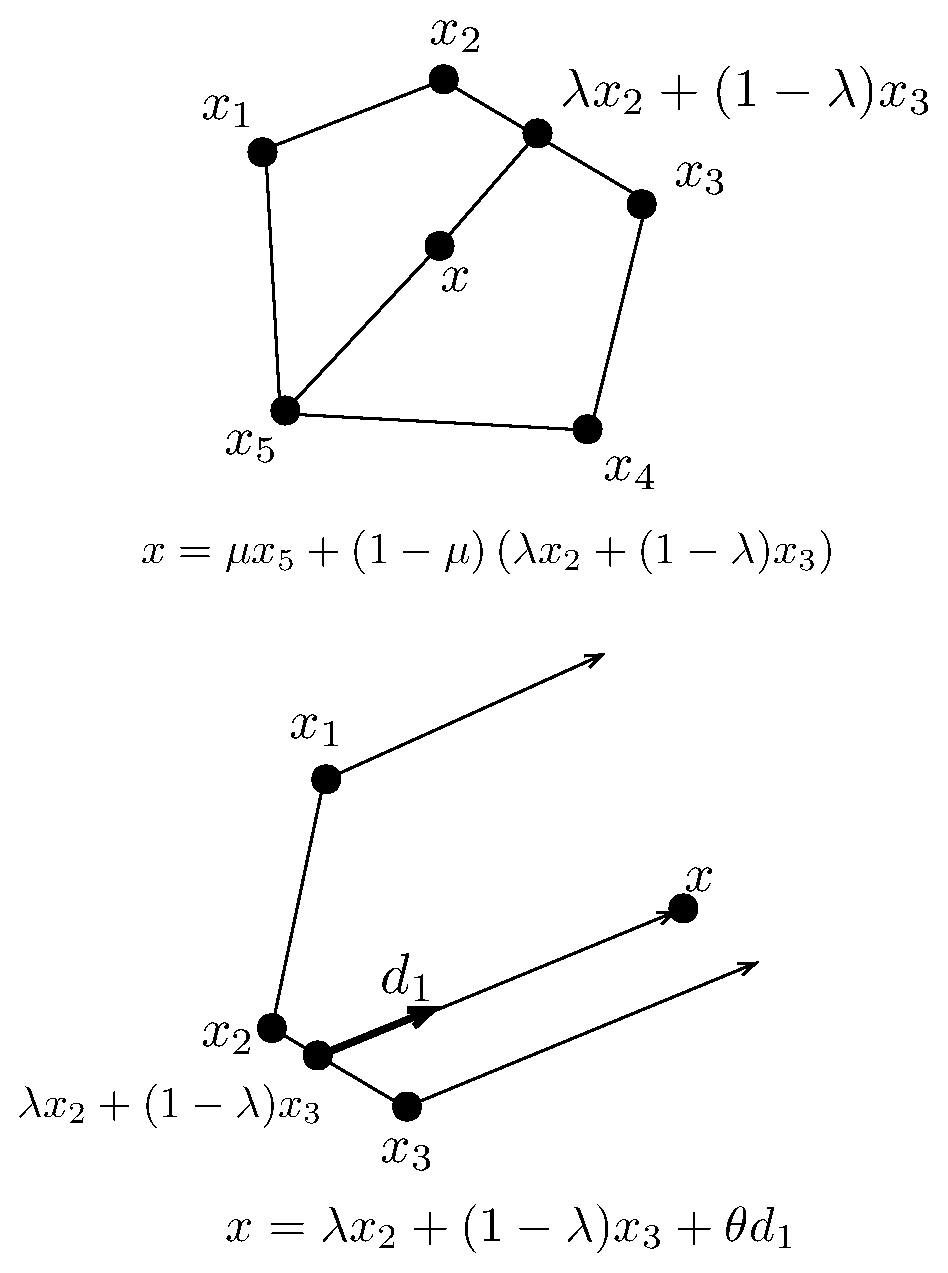
\includegraphics[scale=0.35]{Cartheodoary.pdf}
\caption{The Cartheodory Characterization Theorem: Extreme points and extreme directions are used to express points in a bounded and unbounded set.}
\label{fig:Carth}
\end{figure}
This example illustrates simply how one could construct an expression for an arbitrary point $\mathbf{x}$ inside a polyhedral set in terms of extreme points and extreme directions.
\end{example}
